%%%%%%%%%%%%%%%%%%%%%%%%%%%%%%%%%%%%%%%%%
%
% (c) 2018 by Jennifer Laaser
%
% This work is licensed under the Creative Commons Attribution-NonCommercial-ShareAlike 4.0 International License. To view a copy of this license, visit http://creativecommons.org/licenses/by-nc-sa/4.0/ or send a letter to Creative Commons, PO Box 1866, Mountain View, CA 94042, USA.
%
% The current source for these materials is accessible on Github: https://github.com/jlaaser/pogil-polymers
%
%%%%%%%%%%%%%%%%%%%%%%%%%%%%%%%%%%%%%%%%%

\renewcommand{\figpath}{content/polymchem/stepgrowth/dispersity/figs}

\begin{activity}[Molecular Weight Distributions in Step-Growth Polymerizations]

\begin{instructornotes}

	This activity introduces students to key concepts related to the molecular weight distributions obtained in step-growth polymerizations.
	
	After completing this activity, students will be able to:
			\begin{enumerate}
				\item Calculate the fraction of polymer chains with length $i$ in a step-growth polymerization,
				\item Describe, qualitatively, the chain length distribution and how it changes with extent of reaction,
				\item Calculate the expected dispersity for step-growth polymerizations, and
				\item Explain why the limiting dispersity for a step-growth polymerization is 2.
			\end{enumerate}
			
	\subsection*{Activity summary:}
	\begin{itemize}
		\item \textbf{Activity type:} Learning Cycle
		\item \textbf{Content goals:} Molecular weight distributions and dispersity in step-growth polymerizations
		\item \textbf{Process goals:} %https://pogil.org/uploads/attachments/cj54b5yts006cklx4hh758htf-process-skills-official-pogil-list-2015-original.pdf
			written communication, critical thinking, information processing
		\item \textbf{Duration:} 25-30 minutes, including time for discussion
		\item \textbf{Instructor preparation required:} none beyond knowledge of relevant content
		\item \textbf{Related textbook chapters:}
			\begin{itemize}
				\item \emph{Polymer Chemistry} (Hiemenz \& Lodge): section 2.4
			\end{itemize}
		\item \textbf{Facilitation notes:}
			\begin{itemize}
				\item The process described in Model 1 depicts step-growth polymerizations as a monomer-by-monomer addition process.  Although this simplification was necessary to make the model accessible to students, it is not strictly accurate, since oligomers can react with each other in step-growth polymerizations (and not just with monomers).
			\end{itemize}
	\end{itemize}

\end{instructornotes}

	%\textbf{Focus question:} Put a central question for the students to consider through this exercise here.

\begin{model}[Probabilities of Forming Different Chain Lengths]

To determine the \emph{distribution} of chain lengths formed in a step-growth polymerization, it is useful to calculate the probability of forming each different chain length.

The following diagram summarizes the steps that lead to different chain lengths in a step-growth polymerization of AB-type monomers at extent of reaction $p$:

\vspace{0.1in}
\centerline{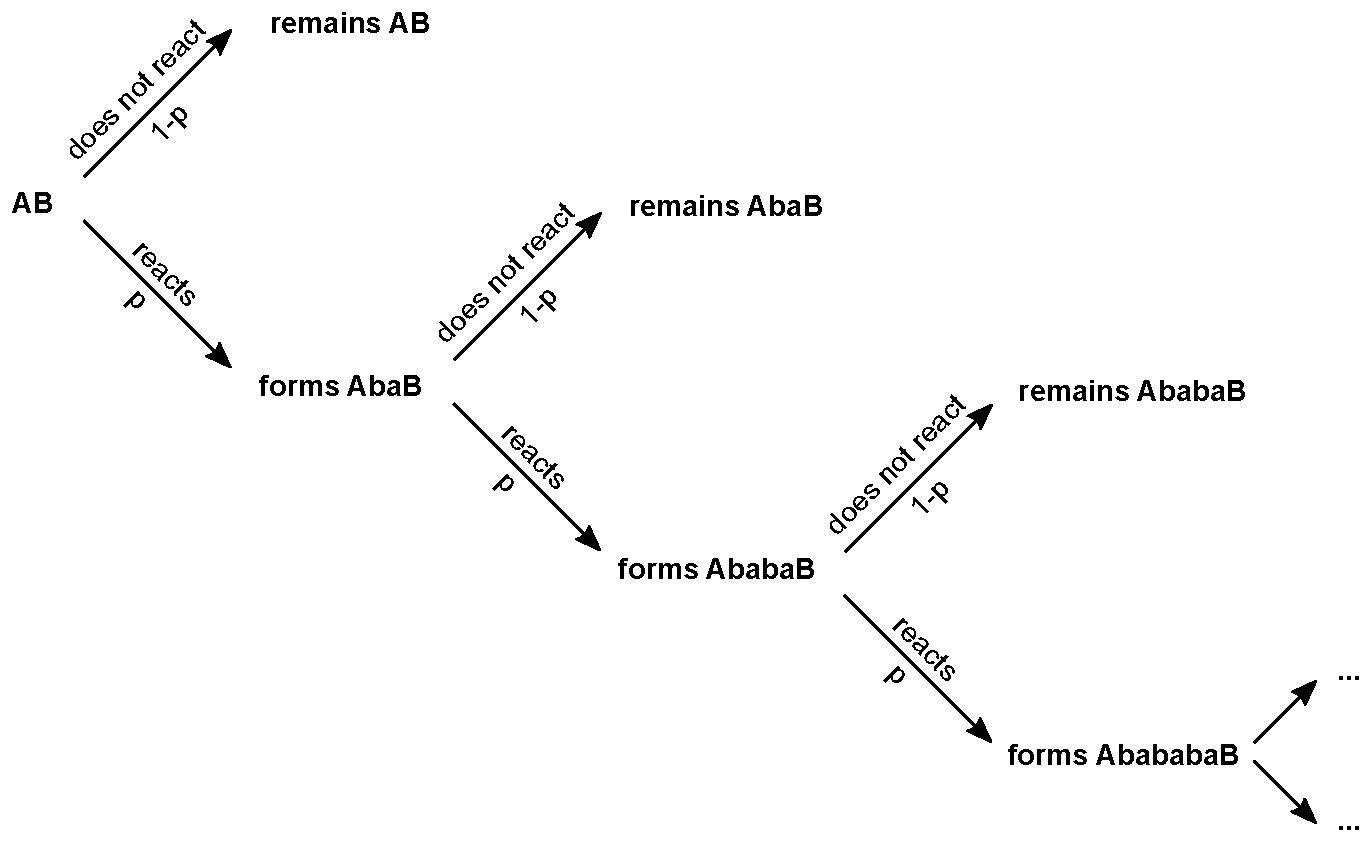
\includegraphics[width=0.9\textwidth]{\figpath/model1-fulltree}}

In this diagram, the different \textbf{states} of the polymer chain are written in bold text.  They are connected by arrows describing the \textbf{processes} that take the chain from one state to the next; the text \emph{above} each arrow describes which process takes place, while the expression \emph{under} each arrow gives the probability of that process occurring.

\end{model}

\vspace{0.05in}
\begin{ctqs}
	
	\question What is the probability that...
	
		\begin{enumerate}
			\item ... an AB monomer does not react, and remains an AB monomer?
	
			\begin{solution}[0.25in]
				$1-p$
			\end{solution}

		\item ... an AB monomer reacts to form an AbaB dimer?
	
			\begin{solution}[0.25in]
				$p$
			\end{solution}
		
		\item ... an AbaB dimer does not react, and remains an AbaB dimer?
	
			\begin{solution}[0.25in]
				$1-p$
			\end{solution}
	
		
		\item ... an AbaB dimer reacts to form an AbabaB trimer?
	
			\begin{solution}[0.25in]
				$p$
			\end{solution}
			
		\end{enumerate}	
		
	\question For \emph{any} molecule with $n$ monomers, what is the probability that it reacts to form a molecule with $n+1$ monomers?
	
			\begin{solution}[0.25in]
				$p$
			\end{solution}
	
	\question Is your answer to the previous question consistent with the definition of the extent of reaction $p$?  Briefly explain your answer in 1-2 complete sentences.
	
		\begin{solution}[2in]
			Yes, it is.  The extent of reaction, $p$, is the fraction of ``A'' groups that have reacted.  Since each molecule has exactly 1 ``A'' group, the fraction of molecules that reach length $n$ whose ``A'' groups react to form chains with $n+1$ monomers is $p$.  This fraction is equivalent to the probability that the chain grows from $n$ to $n+1$ monomers.
		\end{solution}
	
\end{ctqs}

\begin{infobox}

	For a process with a \textbf{single} step, the overall probability of reaching the final state is just the probability of that step.
	
	For example, the series of steps that leads to a chain with exactly one monomer (i.e. an AB monomer that does not react) is shown below:
	
	\vspace{0.1in}
	\centerline{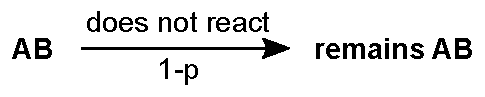
\includegraphics[width=0.3\textwidth]{\figpath/model1-AB}}
	
	Since there is only a single step in this process, the overall probability of obtaining a chain with exactly 1 monomer is just the probability of this step, or $1-p$.
	
	\vspace{0.1in}
	For processes with \textbf{multiple} steps, the overall probability of reaching the final state is the \emph{product} of the probabilities for each step in the process.
	
	For example, the series of steps takes us from an initial AB monomer to an AbaB chain that does not react further (remains a chain with exactly 2 monomers) is:
	
	\vspace{0.1in}
	\centerline{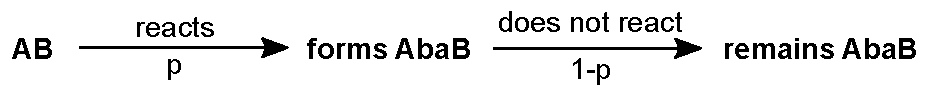
\includegraphics[width=0.6\textwidth]{\figpath/model1-AbaB}}
	
	The first step occurs with probability $p$, while the second step occurs with probability $1-p$; the total probability of obtaining a chain with exactly 2 monomers is the product of these probabilities, or $p(1-p)$.
	
\end{infobox}

\begin{ctqs}

	\question Diagram the series of steps that lead to formation of a chain with 3 monomers that does not react any further:
	
		\begin{solution}[1in]\instructordisplay{
			\centerline{ 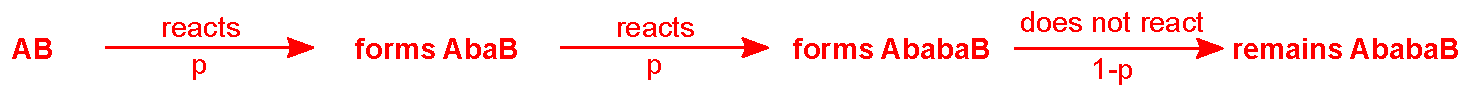
\includegraphics[width=0.8\textwidth]{\figpath/model1-AbabaB-answer}}
		}\end{solution}
	
	\question Based on your diagram, what is the overall probability of obtaining a chain with exactly 3 monomers?
	
		\begin{solution}[1in]
			$p \cdot p \cdot (1-p) = p^2(1-p)$
		\end{solution}
	
	\question Building on this process, fill in the blanks in the following table:
	
		\begin{center}
			\renewcommand{\arraystretch}{3}
			\begin{tabular}{|c|c|}
				\hline
				\textbf{~~i~~} & {\renewcommand{\arraystretch}{1}\begin{tabular}{c}\textbf{Probability that a molecule is composed}\\\textbf{of exactly $i$ monomers}\end{tabular} }\\\hline
				1 & $1-p$\\\hline
				2 & $p(1-p)$\\\hline
				3 & \answer{$p^2(1-p)$}\\\hline
				4 & \answer{$p^3(1-p)$}\\\hline
				5 & \answer{$p^4(1-p)$}\\\hline
			\end{tabular}
		\end{center}
	
	\question What pattern do you notice in these values?  Briefly describe your observations in 1-2 complete sentences.
	
		\begin{solution}[1in]
		
			The values acquire an additional factor of $p$ for each additional monomer in the chain.
		
		\end{solution}
	
	\question Complete the following statement:
	
		``The probability that a molecule is composed of exactly $i$ monomers is \line(1,0){50}.''
	
		\begin{solution}[0.5in]
		
			$p^{i-1}(1-p)$
			
		\end{solution}
		
\end{ctqs}

\begin{infobox}
	The \emph{probability} that a molecule is composed of exactly $i$ monomers is the same as the \emph{fraction of molecules} that are composed of exactly $i$ monomers.
\end{infobox}


\begin{ctqs}
	
	\question Complete the following statement:
	
		``The fraction of molecules, $x_i$, that are composed of exactly $i$ monomers is \line(1,0){50}.''
	
		\begin{solution}[0.5in]
		
			$x_i = p^{i-1}(1-p)$
			
		\end{solution}
	
	\question Using this expression, calculate the fraction of molecules that have exactly length $i$ for both $p=0.5$ and $p=0.9$ at the following values of $i$:
	
		\begin{center}
			\renewcommand{\arraystretch}{3}
			\begin{tabular}{|c|c|c|}
				\hline
				\textbf{~~$i$~~} & ~~~$x_i$ when $p=0.5$~~~ & ~~~$x_i$ when $p=0.9$~~~ \\\hline
				1 & \answer{0.5} & \answer{0.1} \\\hline
				2 & \answer{0.25} & \answer{0.09} \\\hline
				3 & \answer{0.125} & \answer{0.08} \\\hline
				5 & \answer{0.0313} & \answer{0.065} \\\hline
				10 & \answer{9.7x10$^{-4}$} & \answer{0.0387} \\\hline
				15 & \answer{3.1x10$^{-5}$} & \answer{0.0229} \\\hline
				20 & \answer{9.5x10$^{-7}$} & \answer{0.0135} \\\hline
			\end{tabular}
		\end{center}
		
		\clearpage
	\question Plot your results on the following axes.  Make sure to use a different symbol for points corresponding to $p=0.5$ than for the points corresponding to $p=0.9$.
	
		\begin{solution}[2.75in]
			\studentdisplay{
				\centerline{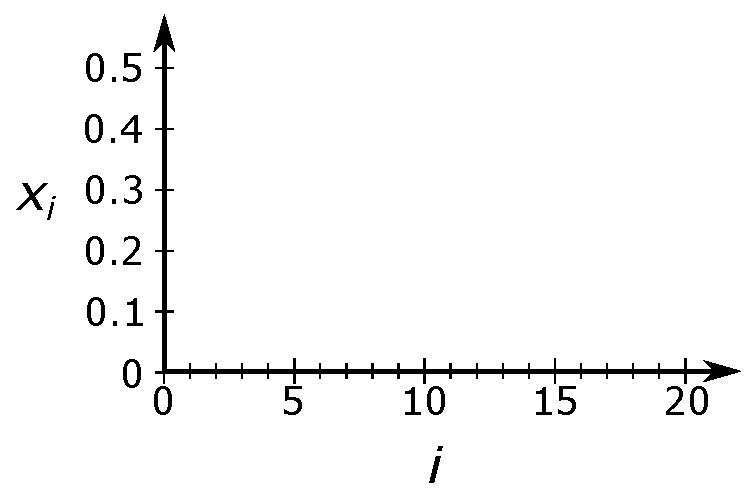
\includegraphics[width=0.7\textwidth]{\figpath/model1-xi-axes.pdf}}
			}
			\instructordisplay{
				\centerline{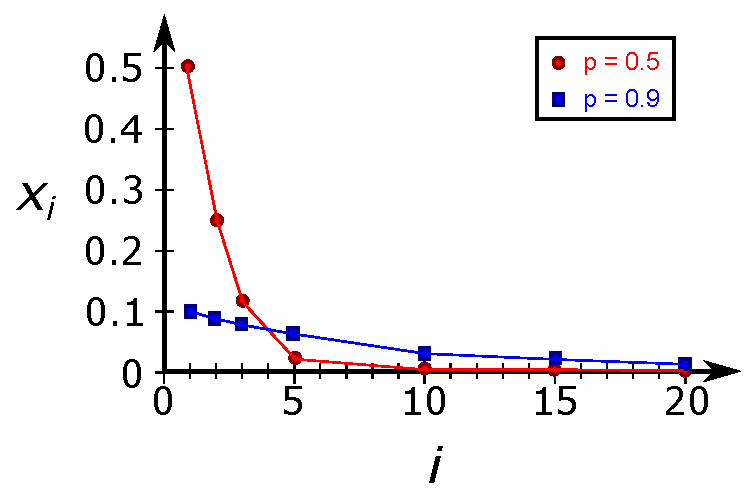
\includegraphics[width=0.7\textwidth]{\figpath/model1-xi-plotted.pdf}}
			}
		\end{solution}
	
	\question How are the plots for $p=0.5$ and $p=0.9$ similar, and how are they different?  Briefly describe your observations in 2-3 complete sentences.
	
		\begin{solution}[1.5in]
		
			Both of these plots decrease exponentially toward zero with increasing values of $i$.  However, the plot for $p=0.5$ decreases much faster, and a higher fraction of the molecules have very short chain lengths, than in the case where $p=0.9$.
		\end{solution}
	
	\question What is the \emph{most probable} chain length for each value of $p$?
	
		\begin{solution}[0.5in]
		
			The most probable chain length is just the one with the highest value of $x_i$.  Thus, the most probably chain length is $i=1$ for both values of $p$.
		
		\end{solution}
	
	\question Can the fraction of chains with length $i+1$ ever be \emph{greater} than the fraction of chains with length $i$?  Justify your answer in 1-2 complete sentences.
	
		\begin{solution}[1.5in]
		
			No, the fraction of chains with length $i+1$ can never be greater than the mole fraction of chains with length $i$.  This is because for each additional monomer, we pick up another factor of $p$; since $p$ is always less than one, $x_{i+1}$ will always be less than $x_i$.
			
			In mathematical terms, $x_i$ decreases monotonically with increasing chain length $i$.
		
		\end{solution}
	
\end{ctqs}


\begin{model}[$M_n$ and $M_w$ for Step-Growth Polymerizations]

	To calculate $M_n$ and $M_w$, we need to know $n_i$, or the total number of chains with $i$ monomers.
	
	If we started with $v_A^0$ monomers, then when the extent of reaction is equal to $p$, there will be $(1-p)v_A^0$ unreacted A groups left.  Recalling that the number of unreacted A groups is equal to the number of molecules in the reaction mixture, this lets us write
	\begin{align*}
		n_i = \text{(fraction of molecules that }&\text{have length }i\text{) x (number of molecules in reaction mixture)}\\
			%&= (x_i)((1-p)v_A^0)\\
			&= \left(p^{i-1}(1-p)\right)\left((1-p)v_A^0\right)\\
			&= p^{i-1}(1-p)^2v_A^0
	\end{align*}
	
	If we plug this expression into our equation for $M_n$, we get
	\begin{equation*}
		M_n = \frac{\sum_i n_i M_i}{\sum_i n_i} %= \frac{\sum_i p^{i-1}(1-p)^2 v_A^0 i M_0}{\sum_i p^{i-1}(1-p)^2 v_A^0} 
		= M_0\frac{\sum_i p^{i-1}(1-p)^2 i }{\sum_i p^{i-1}(1-p)^2}
	\end{equation*}
	where $M_0$ is the molecular weight of the monomer ($M_i = M_0 i$).
	
	\vspace{0.25in}
	
	If we evaluate these sums, we obtain
	\begin{align*}
		M_n = \frac{M_0}{1-p} && \text{or} && N_n = \frac{M_n}{M_0} = \frac{1}{1-p}
	\end{align*}
	which is exactly what we expected (whew - our math worked!).
	
	\vspace{0.25in}
	Similarly, if we plug this expression into our equation for $M_w$ and work through the sums, we get
	\begin{align*}
		M_w = \frac{\sum_i n_i M_i^2}{\sum_i n_i M_i} = M_0\frac{1+p}{1-p} && \text{or} && N_w = \frac{M_w}{M_0} = \frac{1+p}{1-p}
	\end{align*}

\end{model}

\begin{ctqs}
		\question Calculate the dispersity for a step-growth reaction with extent of reaction $p$.
		
			\begin{solution}[1.95in]
			
				\begin{equation*}
					\text{\DJ} = \frac{M_w}{M_n} = \frac{M_0\frac{1+p}{1-p}}{M_0\frac{1}{1-p}} = 1+p
				\end{equation*}
			\end{solution}
			
			
		\question What is the value of the dispersity when $p=0$?  Briefly comment on whether or not this answer makes sense.
		
			\begin{solution}[1.5in]
			
				When $p=0$, $\text{\DJ}=1+0 = 1$.  This does make sense: when the extent of reaction is zero, no reactions have taken place, and the reaction mixture contains only monomers.  Since all of the molecules in the mixture are thus identcail (and exactly the same size), the dispersity is 1 - the mixture is monodisperse.
			
			\end{solution}
			
			
		\question What is the value of the dispersity when $p=1$?
		
			\begin{solution}[1in]
			
				When $p=1$, $\text{DJ}=1+1=2$.  This is an important limit: the limiting dispersity for a step-growth polymerization is 2.
			
			\end{solution}
			
			
			
		\question Can the dispersity of a polymer produced by step-growth polymerization ever be greater than 2?  Briefly defend your answer in 1-2 complete sentences.
		
			\begin{solution}[1.5in]
			
				Following the argument presented in this exercise, no, the dispersity of a polymer produced by step-growth polymerization can never be greater than 2, because $p$ can never be greater than 1. 
				
				Note for instructors: practically speaking, there are certain conditions that can generate dispersities greater than 2 (for example, when the reaction mixture contains multifunctional monomers that induce chain branching, or when the monomers are added in several batches - see DOI:10.1016/0032-3861(92)90340-3), but for the purposes of this activity, students should learn that the ideal limiting dispersity for step-growth polymerizations is two.
			
			\end{solution}
			
			
\end{ctqs}

\begin{exercises}

		\exercise Suppose you synthesized a polymer by step-growth polymerization and found that it had a dispersity of 1.86.
		
			\begin{enumerate}
				\item What must the extent of reaction have been in this polymerization?
		
					\begin{solution}
					\instructordisplay{
						\begin{equation*}
							p = \text{\DJ}-1 = 1.86-1 = 0.86
						\end{equation*}
					}
					\end{solution}
					
				\item What would you expect the number-average degree of polymerization of this polymer to be?
		
					\begin{solution}
					\instructordisplay{
						\begin{equation*}
							N_n = \frac{1}{1-p} = \frac{1}{1-0.86} = 7.1
						\end{equation*}
					}
					\end{solution}
			\end{enumerate}
			
		\exercise Show that the summation expression for $M_n$ given in Model 2 simplifies to the expected result by doing the following:
		
			\begin{enumerate}
				\item First, show that the summation expression for $M_n$ given in Model 2 can be rewritten
					\begin{equation*}
						M_n = M_0 \frac{{\sum_i i p^{i-1}}}{\frac{1}{p}\sum_i p^i}
					\end{equation*}
					
					\begin{solution}\instructordisplay{
						In Model 2, $M_n$ was written as
						\begin{equation*}
							M_n = M_0\frac{\sum_i p^{i-1}(1-p)^2 i }{\sum_i p^{i-1}(1-p)^2}
						\end{equation*}
						We can simplify this by realizing that any multiplicative terms that do not depend on $i$ can be pulled out of the sum:
						\begin{equation*}
							M_n = M_0\frac{(1-p)^2\sum_i p^{i-1} i }{(1-p)^2\sum_i p^{i-1}} = M_0\frac{\sum_i p^{i-1} i }{\sum_i p^{i-1}}
						\end{equation*}
						Similarly, using $p^{i-1} = p^i/p$,
						\begin{equation*}
							M_n = M_0\frac{\sum_i p^{i-1} i }{\sum_i p^{i-1}} = M_0\frac{\sum_i p^{i-1} i }{\frac{1}{p}\sum_i p^{i}}
						\end{equation*}
						
					}\end{solution}
					
				\item The denominator of this expression is just a geometric series.  Recall that if $p < 1$, then 
		
			\begin{equation*}
				\sum_{i=1}^{\infty} p^i = \frac{p}{1-p}
			\end{equation*}
			
					Substitute this expression into your equation for $M_n$ and simplify.
					
					\begin{solution}\instructordisplay{
						\begin{align*}
							M_n &= M_0\frac{\sum_i p^{i-1} i }{\frac{1}{p}\sum_i p^{i}}\\
								&= M_0\frac{\sum_i p^{i-1} i }{\frac{1}{p}\frac{p}{1-p}}\\
								&= M_0 (1-p)\sum_i p^{i-1} i 
						\end{align*}
						
					}\end{solution}
			
				\item The remaining sum can be calculated by differentiating both sides of the equation for $\sum_i p^i$.  Carry out this differentiation to show that
						\begin{equation*}
							\sum_{i=1}^{\infty} ip^{i-1} = \frac{1}{(1-p)^2}
						\end{equation*}
				
					\begin{solution}\instructordisplay{
						Left-hand side:
						\begin{align*}
							\frac{d}{dp} \sum_{i=1}^{\infty} p^i &= \sum_{i=1}^{\infty} \frac{d}{dp} p^i\\
							&= \sum_{i=1}^{\infty} ip^{i-1}
						\end{align*}
						Note that the derivative can move through the sum since the derivative depends only on $p$, not $i$.
						
						Right-hand side:
						\begin{align*}
							\frac{d}{dp} \frac{p}{1-p} &= \frac{d}{dp} p(1-p)^{-1}\\
							&= p\frac{d}{dp}(1-p)^{-1} + (1-p)^{-1}\frac{d}{dp} p\\
							&= p(1-p)^{-2} + (1-p)^{-1}\\
							&= \frac{1}{1-p}\left(\frac{p}{1-p} + 1\right)\\
							&= \frac{1}{1-p}\left(\frac{p + 1 - p}{1-p}\right)\\
							&= \frac{1}{1-p}\left(\frac{1}{1-p}\right)\\
							&= \frac{1}{(1-p)^2}
						\end{align*}
						
						Setting them equal, we obtain:
						\begin{equation*}
							\sum_{i=1}^{\infty} ip^{i-1} = \frac{1}{(1-p)^2}
						\end{equation*}
						
					}\end{solution}
					
				\item Finally, substitute this expression into $M_n$ and show that you obtain the expected solution.
				
				
					\begin{solution}\instructordisplay{
						\begin{align*}
							M_n &= M_0 (1-p)\sum_i p^{i-1} i \\
								&= M_0 (1-p)\frac{1}{(1-p)^2} \\
								&= M_0 \frac{1}{1-p}
						\end{align*}
						as expected.
					}\end{solution}
				
			\end{enumerate}
			
\end{exercises}
	
\end{activity}